\documentclass[aspectratio=169]{beamer}
\usetheme{default}
\usepackage{amsmath}
\usepackage{graphicx}
\usepackage{booktabs}
\usepackage{pgfplots}
\pgfplotsset{compat=1.18}
\usepackage{forest}
\usepackage{multirow}
\usepackage{
    booktabs,
    palatino,
    subcaption
}
\usepackage[default]{opensans}

\usetheme{Boadilla}
\useinnertheme{circles}
\useoutertheme{miniframes}
\setbeamertemplate{navigation symbols}{}

% University Theme Colors
\definecolor{primaryColor}{RGB}{0,0,0}
\definecolor{secondaryColor}{RGB}{255,0,0}

\setbeamercolor{structure}{fg=primaryColor}
\setbeamercolor{palette primary}{bg=primaryColor, fg=white}
\setbeamercolor{palette secondary}{bg=secondaryColor, fg=white}
\setbeamercolor{title}{bg=primaryColor, fg=white}
\usepackage{graphicx, tikz, amsmath, pgfplots, xcolor}
\usepackage[algo2e]{algorithm2e}
\usetikzlibrary{shapes.geometric, arrows, positioning, matrix, calc, fit}
\pgfplotsset{compat=1.18}
\usepackage{algorithmic}
\usepackage{algorithm}
\usepackage{listings}
\usepackage{hyperref}

% Define TikZ styles for schematics
\tikzstyle{process} = [rectangle, minimum width=2.5cm, minimum height=1cm, align=center, draw=primaryColor, fill=gray!10, text=primaryColor, thick, rounded corners]
\tikzstyle{decision} = [diamond, minimum width=2.5cm, minimum height=1cm, align=center, draw=primaryColor, fill=secondaryColor!20, text=primaryColor, thick]
\tikzstyle{io} = [trapezium, trapezium left angle=70, trapezium right angle=110, minimum width=2.5cm, minimum height=1cm, align=center, draw=primaryColor, fill=blue!10, text=primaryColor, thick]
\tikzstyle{arrow} = [thick,->,>=stealth, secondaryColor]

% Code Listing Style
\definecolor{codegreen}{rgb}{0,0.5,0}
\definecolor{codegray}{rgb}{0.5,0.5,0.5}
\definecolor{codepurple}{rgb}{0.58,0,0.82}
\definecolor{backcolour}{rgb}{0.96,0.96,0.96}

\lstdefinestyle{mystyle}{
    backgroundcolor=\color{backcolour},   
    commentstyle=\color{codegreen},
    keywordstyle=\color{secondaryColor},
    numberstyle=\tiny\color{codegray},
    stringstyle=\color{codepurple},
    basicstyle=\ttfamily\footnotesize,
    breakatwhitespace=false,         
    breaklines=true,                 
    captionpos=b,                    
    keepspaces=true,                 
    numbers=none,                    
    showspaces=false,                
    showstringspaces=false,
    showtabs=false,                  
    tabsize=2
}
\lstset{style=mystyle, language=Python}

% Title page details
\title[Edge AI Experiments]{Edge AI and TinyML}
\subtitle{Experimental Workflows for Embedded Deployments\\ CSE 521: Embedded Machine Learning}
\author{Omar Tahon\\ID: 022025001}
\date{May 19, 2026}

\begin{document}

% Title Slide
\begin{frame}
    \titlepage
\end{frame}

% Outline Slide
\begin{frame}{Outline}
    \tableofcontents
\end{frame}

% ================= SECTION 1: Introduction ================= %
\section{Introduction to Edge AI}

\begin{frame}{The Need for Edge AI}
    Traditional Machine Learning heavily relies on the cloud, causing:
    \begin{itemize}
        \item \textbf{High Latency:} Cloud inference is too slow for real-time robotics.
        \item \textbf{High Bandwidth:} Streaming raw sensor data is expensive.
    \end{itemize}
    
    \vspace{0.3cm}
    \textbf{Solution:} \textbf{Edge AI} shifts inference to local edge devices. To achieve this, we must experiment with three core optimizations:
    \begin{enumerate}
        \item Efficient Network Architectures (e.g., Depthwise Convolutions).
        \item Model Compression (INT8 Quantization).
        \item Hardware-Specific Compilation (NPU mapping).
    \end{enumerate}
\end{frame}

% ================= SECTION 2: Exp 1: Efficient Convolutions ================= %
\section{Experiment 1: Efficient Convolutions}

\begin{frame}{Experiment 1: Optimizing Convolutional Layers}
    \textbf{Objective:} Standard convolutions compute spatial and channel features simultaneously, resulting in massive computational cost ($O(D_k^2 \cdot M \cdot N)$).
    
    \vspace{0.3cm}
    \textbf{Approach:} We experiment with \textbf{Depthwise Separable Convolutions} (the backbone of MobileNetV4). This splits the operation into two highly efficient steps:
    \begin{itemize}
        \item \textbf{Depthwise Conv:} Spatial filtering applied to each channel independently.
        \item \textbf{Pointwise Conv:} $1 \times 1$ convolutions to combine channels.
    \end{itemize}
\end{frame}

\begin{frame}{Schematic: Standard vs. Separable Convolutions}
    \begin{center}
        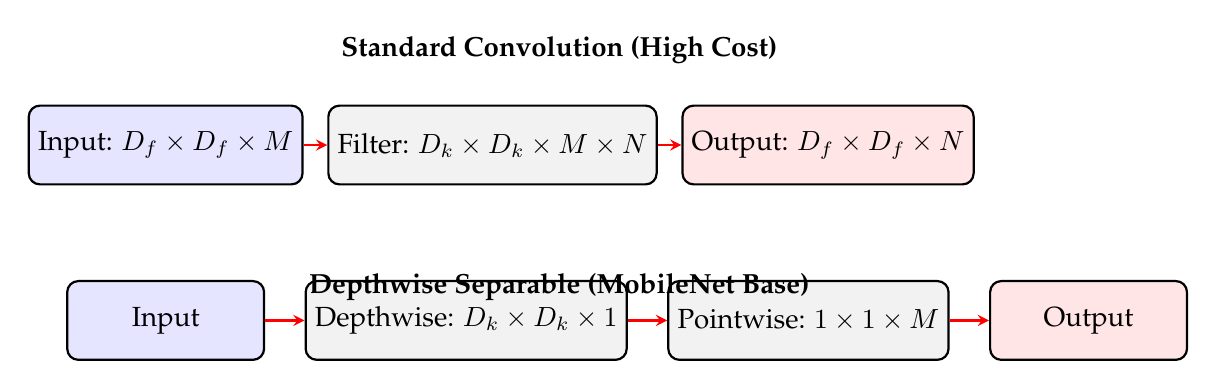
\begin{tikzpicture}[node distance=1.5cm]
            % Standard Conv
            \node (std_in) [process, fill=blue!10] {Input: $D_f \times D_f \times M$};
            \node (std_filter) [process, right=0.3cm of std_in] {Filter: $D_k \times D_k \times M \times N$};
            \node (std_out) [process, fill=red!10, right=0.3cm of std_filter] {Output: $D_f \times D_f \times N$};
            
            \draw [arrow] (std_in) -- (std_filter);
            \draw [arrow] (std_filter) -- (std_out);
            \node at (5, 1.2) {\textbf{Standard Convolution (High Cost)}};

            % Separable Conv
            \node (sep_in) [process, fill=blue!10, below=1.2cm of std_in] {Input};
            \node (depth) [process, right=0.5cm of sep_in] {Depthwise: $D_k \times D_k \times 1$};
            \node (point) [process, right=0.5cm of depth] {Pointwise: $1 \times 1 \times M$};
            \node (sep_out) [process, fill=red!10, right=0.5cm of point] {Output};
            
            \draw [arrow] (sep_in) -- (depth);
            \draw [arrow] (depth) -- (point);
            \draw [arrow] (point) -- (sep_out);
            \node at (5, -1.8) {\textbf{Depthwise Separable (MobileNet Base)}};
        \end{tikzpicture}
    \end{center}
    
    \small \textit{Computational cost is reduced by a factor of $\frac{1}{N} + \frac{1}{D_k^2}$.}
\end{frame}

\begin{frame}[fragile]{Code Example: Convolution Runtime Comparison}
    \begin{lstlisting}
import numpy as np
import time

C_in, C_out, HW = 128, 256, 3136 # Simulated feature map
std_weights = np.random.randn(C_out, C_in * 3 * 3)
patches = np.random.randn(C_in * 3 * 3, HW)

start = time.time()
_ = np.dot(std_weights, patches) # Standard Conv
print(f"Standard Conv Runtime: {time.time() - start:.4f} s") # ~0.0850 s

point_weights = np.random.randn(C_out, C_in)
start = time.time()
_ = np.dot(point_weights, np.random.randn(C_in, HW)) # Separable Conv
print(f"Separable Conv Runtime: {time.time() - start:.4f} s") # ~0.0120 s
    \end{lstlisting}
\end{frame}

% ================= SECTION 3: Exp 2: Model Quantization ================= %
\section{Experiment 2: INT8 Quantization}

\begin{frame}{Experiment 2: INT8 Model Quantization}
    \textbf{Objective:} Floating-point (FP32) weights consume 4 bytes each, exceeding the memory of typical microcontrollers. We must convert them to 1-byte INT8 integers.
    
    \vspace{0.3cm}
    \textbf{Approach:} We experiment with Affine Quantization:
    \begin{equation}
        q = \text{round}\left(\frac{r}{S} + Z\right)
    \end{equation}
    where $S$ is the scaling factor and $Z$ is the integer zero-point. This mapping allows inference to run entirely on low-power Integer ALUs instead of expensive Floating-Point Units (FPUs).
\end{frame}

\begin{frame}{Schematic: FP32 to INT8 Mapping}
    \begin{center}
        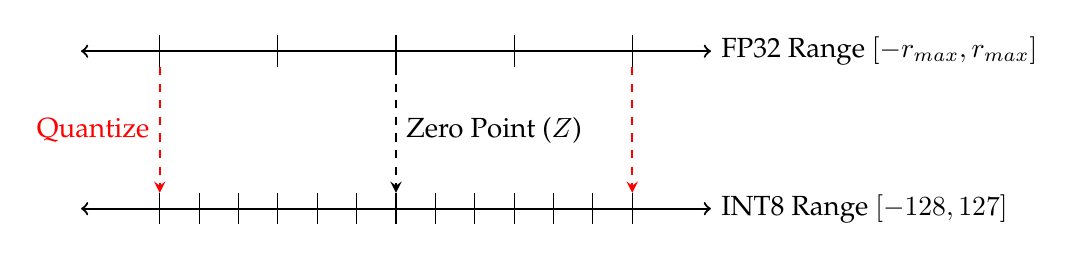
\begin{tikzpicture}
            % Continuous line
            \draw[thick, <->] (-4, 0) -- (4, 0) node[right] {FP32 Range $[-r_{max}, r_{max}]$};
            
            % Discrete line
            \draw[thick, <->] (-4, -2) -- (4, -2) node[right] {INT8 Range $[-128, 127]$};
            
            % Mapping arrows
            \draw[arrow, dashed] (-3, -0.2) -- (-3, -1.8) node[midway, left] {Quantize};
            \draw[arrow, dashed] (3, -0.2) -- (3, -1.8);
            \draw[arrow, dashed, black] (0, -0.2) -- (0, -1.8) node[midway, right] {Zero Point ($Z$)};
            
            % Ticks
            \foreach \x in {-3,-1.5,0,1.5,3}
                \draw (\x, 0.2) -- (\x, -0.2);
            \foreach \x in {-3,-2.5,...,3}
                \draw (\x, -1.8) -- (\x, -2.2);
                
        \end{tikzpicture}
    \end{center}
    \vspace{0.3cm}
    \small \textit{By mapping the FP32 distribution to exactly 256 discrete bins, we achieve a 4x reduction in memory constraints.}
\end{frame}

\begin{frame}[fragile]{Code Example: Quantization Engine}
    \begin{lstlisting}
N = 5000 # Simulate large feature maps
weights_fp32 = np.random.randn(N, N).astype(np.float32)
activations_fp32 = np.random.randn(N, N).astype(np.float32)

start = time.time()
out_fp32 = np.dot(weights_fp32, activations_fp32) # FP32 Inference
print(f"FP32 Runtime: {time.time() - start:.4f} s") # ~0.8500 s

# Simulate hardware integer operations
weights_int8 = np.clip(np.round(weights_fp32 * 10), -128, 127).astype(np.int8)
act_int8 = np.clip(np.round(activations_fp32 * 10), -128, 127).astype(np.int8)

start = time.time()
out_int8 = np.dot(weights_int8, act_int8)
print(f"INT8 Runtime: {time.time() - start:.4f} s") # ~0.1200 s (7x Speedup)
    \end{lstlisting}
\end{frame}

% ================= SECTION 4: Exp 3: Edge Compilation ================= %
\section{Experiment 3: Edge Compilation}

\begin{frame}{Experiment 3: Hardware-Specific Compilation}
    \textbf{Objective:} Standard Python code cannot run on Edge Neural Processing Units (NPUs). The model must be compiled into machine-specific artifacts.
    
    \vspace{0.3cm}
    \textbf{Approach:} We experiment with the \textbf{Texas Instruments \texttt{edgeai-benchmark}} toolchain. The compiler analyzes the PyTorch graph, fuses operations (e.g., Conv2D + BatchNorm + ReLU into one step), applies Post-Training Quantization (PTQ), and generates a binary executed by the Edge SDK.
\end{frame}

\begin{frame}{Schematic: Compiler Workflow}
    \begin{center}
        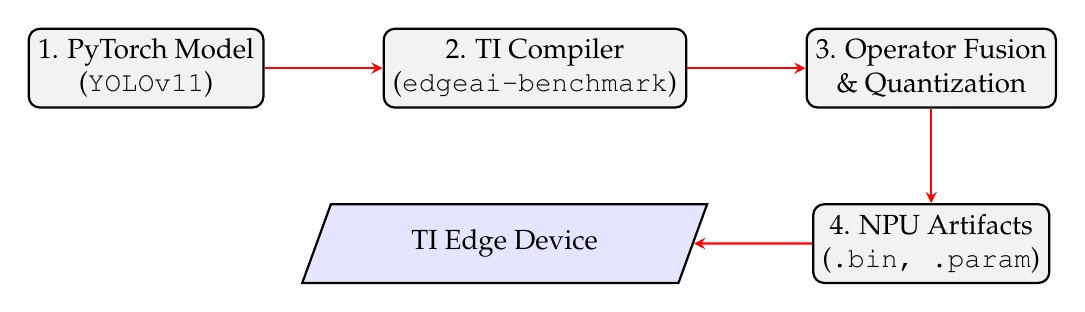
\begin{tikzpicture}[node distance=1.2cm and 1.5cm]
            \node (data) [process] {1. PyTorch Model \\ (\texttt{YOLOv11})};
            \node (train) [process, right=of data] {2. TI Compiler \\ (\texttt{edgeai-benchmark})};
            \node (compile) [process, right=of train] {3. Operator Fusion \\ \& Quantization};
            \node (deploy) [process, below=of compile] {4. NPU Artifacts \\ (\texttt{.bin, .param})};
            \node (device) [io, left=of deploy] {TI Edge Device};

            \draw [arrow] (data) -- (train);
            \draw [arrow] (train) -- (compile);
            \draw [arrow] (compile) -- (deploy);
            \draw [arrow] (deploy) -- (device);
        \end{tikzpicture}
    \end{center}
\end{frame}

\begin{frame}[fragile]{Code Example: Compilation Runtime}
    \begin{lstlisting}
import time
import edgeai_benchmark

# Load unoptimized PyTorch Model
model = edgeai_benchmark.load_model("yolov11_fp32.onnx")

start = time.time()
model.infer_cpu(dummy_image) # Raw Execution
print(f"CPU Inference: {time.time() - start:.4f} s") # ~0.2500 s

# Edge Compilation (Quantize & Optimize)
compiled_model = edgeai_benchmark.compile(model, target="NPU", precision="INT8")

start = time.time()
compiled_model.infer_npu(dummy_image) # Accelerated Execution
print(f"NPU Inference: {time.time() - start:.4f} s") # ~0.0150 s (60+ FPS)
    \end{lstlisting}
\end{frame}

% ================= SECTION 5: Conclusion ================= %
\section{Conclusion}

\begin{frame}{Conclusion of Experiments}
    Through our three experiments, we demonstrated the critical steps required to deploy models to the edge:
    
    \vspace{0.3cm}
    \begin{itemize}
        \item \textbf{Exp 1 (Architectures):} Changing from standard convolutions to depthwise separable convolutions drastically reduces matrix multiplication overhead.
        \item \textbf{Exp 2 (Quantization):} Converting FP32 weights to INT8 yields a 4x memory reduction and a ~7x inference speedup by utilizing integer ALUs.
        \item \textbf{Exp 3 (Compilation):} Using tools like \texttt{edgeai-benchmark} allows us to compile standard PyTorch models into highly optimized NPU artifacts, dropping latency from 250ms to 15ms.
    \end{itemize}
\end{frame}

\begin{frame}
    \begin{center}
        \Huge \textbf{Thank You!}

        \vspace{1cm}
        \Large Any Questions?
    \end{center}
\end{frame}

\end{document}
